\section{Tests}

(TODO) Vervollst"andigen

Die Tests, die w�hrend der Fachstudie in Nexus-Labor mit der Test-Hardware 
durchgef�hrt wurden, sind in diesen Abschnitt detalliert beschrieben.

%%%%%%%%%%%%%%%%%%%%%%%%%%%%%%%%%%%%%%%%%%%%%%%%%%%%%%%%%%%%%%%%%%%%%%%%%%%%
%
% Erster Test
%
%%%%%%%%%%%%%%%%%%%%%%%%%%%%%%%%%%%%%%%%%%%%%%%%%%%%%%%%%%%%%%%%%%%%%%%%%%%%
\subsection{Erster Test}

%%%%%%%%%%%%%%%%%%%%%%%%%%%%%%%%%%%%%%%%%%%%%%%%%%%%%%%%%%%%%%%%%%%%%%%%%%%%
% Hardware
%%%%%%%%%%%%%%%%%%%%%%%%%%%%%%%%%%%%%%%%%%%%%%%%%%%%%%%%%%%%%%%%%%%%%%%%%%%%
\subsubsection{Hardware}

Zuerst wurde folgende Hardware f"ur den Tests im Nexus-Labor eingerichtet:

\begin{itemize}
	\item Zwei PCs mit \emph{Wistron CM9 Atheros AR5213A} Wlan Karten
  \item Ein Laptop mit Intel mini-PCI Wlan Karte
\end{itemize}

%\wlanimage{Labor}{Topologie}
\begin{figure}[H]
  \centering
  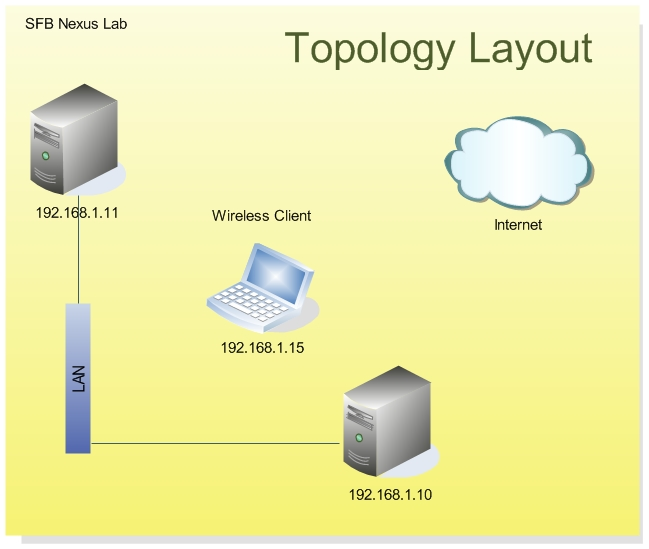
\includegraphics[width=0.8\textwidth]{images/Labor.jpg}
  \caption{Topologie}
  \label{fig:Topologie}
\end{figure}

%%%%%%%%%%%%%%%%%%%%%%%%%%%%%%%%%%%%%%%%%%%%%%%%%%%%%%%%%%%%%%%%%%%%%%%%%%%%
% Software
%%%%%%%%%%%%%%%%%%%%%%%%%%%%%%%%%%%%%%%%%%%%%%%%%%%%%%%%%%%%%%%%%%%%%%%%%%%%
\subsubsection{Software}

Dann wurde Betriebsystem Linux (Fedora 2.6.18) auf den Rechnern installiert.
%%%%%%%%%%%%%%%%%%%%%%%%%%%%%%%%%%%%%%%%%%%%%%%%%%%%%%%%%%%%%%%%%%%%%%%%%%%%
%
% Madwifi
%
%%%%%%%%%%%%%%%%%%%%%%%%%%%%%%%%%%%%%%%%%%%%%%%%%%%%%%%%%%%%%%%%%%%%%%%%%%%%
\paragraph{Madwifi}

Danach wurden die Linux-Treiber Madwifi installiert: 
(\emph{Treiber sind nur f"ur Fedora 2.6.18 kernel!})

Die einzelnen Schritte dabei waren:

\textbf{1. Treiber installieren}
\begin{verbatim}
			# svn checkout http://svn.madwifi.org/madwifi/trunk madwifi	
			# cd madwifi	
			# make	
			# make install
\end{verbatim}

\textbf{2a. Treiber laden manuell}
\begin{verbatim}
			# modprobe ath_pci
\end{verbatim}

\textbf{2b. Treiber laden automatisch}
\begin{verbatim}
			# mkdir /etc/modules.autoload.d/
			# echo ath_pci >> /etc/modules.autoload.d/kernel-2.6
\end{verbatim}

\textbf{3a. Network-Config manuel}
\begin{verbatim}
			# iwlist ath1 frequency	
			          Channel 01 : 2.412 GHz
			          Channel 02 : 2.417 GHz
			          Channel 03 : 2.422 GHz
			          Channel 04 : 2.427 GHz
			          Channel 05 : 2.432 GHz
			          Channel 06 : 2.437 GHz
			          Channel 07 : 2.442 GHz
			          Channel 08 : 2.447 GHz
			          Channel 09 : 2.452 GHz
			          Channel 10 : 2.457 GHz
			          Channel 11 : 2.462 GHz
			          Channel 36 : 5.18 GHz
			          Channel 40 : 5.2 GHz
			          Channel 42 : 5.21 GHz
			          Channel 44 : 5.22 GHz
			          Channel 48 : 5.24 GHz
			          Channel 50 : 5.25 GHz
			          Channel 52 : 5.26 GHz
			          Channel 56 : 5.28 GHz
			          Channel 58 : 5.29 GHz
			          Channel 60 : 5.3 GHz
			          Channel 64 : 5.32 GHz
			          Channel 149 : 5.745 GHz
			          Channel 152 : 5.76 GHz
			          Channel 153 : 5.765 GHz
			          Channel 157 : 5.785 GHz
			          Channel 160 : 5.8 GHz
			          Channel 161 : 5.805 GHz
			          Channel 165 : 5.825 GHz
			          Current Channel=0	
			          
			# ifconfig ath1 inet 192.168.0.1/24	
			# iwconfig ath1 essid mesh
			# iwconfig ath1 mode ad-hoc
			# iwconfig ath1 channel 36
			# iwconfig ath1 enc n1e2x3u4s5
\end{verbatim}

\textbf{3b. Network-Config automatisch}
Datei erstellen:

\begin{verbatim}
			# mkdir /etc/sysconfig/network-scripts/ifcfg-ath1
\end{verbatim}

und editieren..

\begin{verbatim}
			# Silicon Integrated Systems [SiS] SiS900 PCI Fast Ethernet
			DEVICE=ath1
			ONBOOT=yes
			
			BOOTPROTO=static
			IPADDR=192.168.2.1x
			NETMASK=255.255.255.0
			
			ESSID=mesh
			MODE=ad-hoc
			CHANNEL=36 # 5.18 GHz
			KEY=s:0nexus0suxen0
			# 108-Bit WEP 13 zeichen
\end{verbatim}
%%%%%%%%%%%%%%%%%%%%%%%%%%%%%%%%%%%%%%%%%%%%%%%%%%%%%%%%%%%%%%%%%%%%%%%%%%%%
%
% OLSR Daemon
%
%%%%%%%%%%%%%%%%%%%%%%%%%%%%%%%%%%%%%%%%%%%%%%%%%%%%%%%%%%%%%%%%%%%%%%%%%%%%
\paragraph{OLSR Daemon}

Nach der Installation von Madwifi wurde olsrd Daemon 
installiert und konfiguriert:

\textbf{1. olsrd installieren}
\begin{verbatim}
			# cvs -d:pserver:anonymous@olsrd.cvs.sourceforge.net:/cvsroot/olsrd login
			# cvs -z3 -d:pserver:anonymous@olsrd.cvs.sourceforge.net:/cvsroot/olsrd co olsrd-current
			# cd olsrd-current
			# make
			# make install
\end{verbatim}

\textbf{2. Plug-ins f"ur olsrd installieren }
\begin{verbatim}
			# cd lib/"plugin-name"
			# make 
			# make install 
			# chcon -t textrel_shlib_t /usr/lib/olsrd_httpinfo.so.0.1 (!)
\end{verbatim}

\textbf{3. olsrd kofigurieren}

\begin{itemize}
	\item Datei /etc/olsrd.conf erstellen und editieren!!! (TODO) (LINK) Anhang (sieh file) 
	\item TCP Port 8080 f"ur Httpinfo und 8081 f"ur Dot UDP 698 f"ur Eingehende 
				Pakete erlauben. 
	\item Datei /etc/sysconfig/iptables editieren: 
\end{itemize}

\begin{verbatim}
			-A RH-Firewall-1-INPUT -p tcp --dport 8080 -m state --state NEW -j ACCEPT
			-A RH-Firewall-1-INPUT -p tcp --dport 8081 -m state --state NEW -j ACCEPT
			-A RH-Firewall-1-INPUT -i ath1 -p udp --sport 698 -j ACCEPT
\end{verbatim}

\textbf{4. olsrd starten }
\begin{verbatim}
 			# olsrd
\end{verbatim}

%%%%%%%%%%%%%%%%%%%%%%%%%%%%%%%%%%%%%%%%%%%%%%%%%%%%%%%%%%%%%%%%%%%%%%%%%%%%
%
% Ergebnisse
%
%%%%%%%%%%%%%%%%%%%%%%%%%%%%%%%%%%%%%%%%%%%%%%%%%%%%%%%%%%%%%%%%%%%%%%%%%%%%
\subsubsection{Ergebnisse}
(TODO) korrigieren
\paragraph{Topologie}
Mittels \emph{olsrd-Plugin dot}, wurde folgende Topologie-Abbildung erstellt.
(TODO) Beschreiben..
\wlanimage{Topology}{Topologie Graph}

\paragraph{Http Info}
Mittels \emph{olsrd-Plugin Http Info}, wurde folgende Routing-"Ubersicht-Abbildung erstellt.
(TODO) Beschreiben..

\begin{figure}[H]
  \centering
  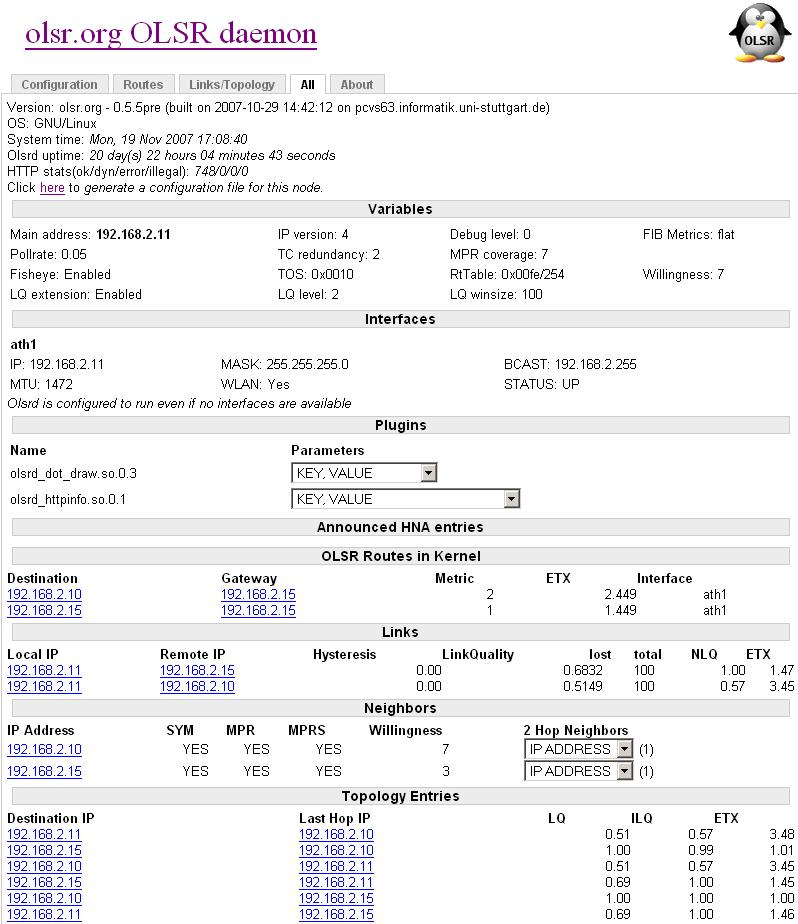
\includegraphics[width=1.0\textwidth]{images/Olsr_Route.jpg}
  \caption{Http Info}
  \label{fig:Olsr_Route}
\end{figure}

%%%%%%%%%%%%%%%%%%%%%%%%%%%%%%%%%%%%%%%%%%%%%%%%%%%%%%%%%%%%%%%%%%%%%%%%%%%%
%
% Zweiter Test
%
%%%%%%%%%%%%%%%%%%%%%%%%%%%%%%%%%%%%%%%%%%%%%%%%%%%%%%%%%%%%%%%%%%%%%%%%%%%%
\subsection{Zweiter Test}

(TODO) .. 2 laptops, windows, ..